% Template for ICASSP-2018 paper; to be used with:
%          spconf.sty  - ICASSP/ICIP LaTeX style file, and
%          IEEEbib.bst - IEEE bibliography style file.
% --------------------------------------------------------------------------
\documentclass{article}
\usepackage{spconf,amsmath,graphicx,hyperref}
\usepackage{caption,subcaption}

% Example definitions.
% --------------------
\def\x{{\mathbf x}}
\def\L{{\cal L}}

% Title.
% ------
\title{AUTHOR GUIDELINES FOR ICASSP 2018 PROCEEDINGS MANUSCRIPTS}
%
% Single address.
% ---------------
\name{Mattia Lecci, Federico Mason, Victor Cercos Llombart}
\address{UPC ETSETB - MET}
%
% For example:
% ------------
%\address{School\\
%	Department\\
%	Address}
%
% Two addresses (uncomment and modify for two-address case).
% ----------------------------------------------------------
%\twoauthors
%  {A. Author-one, B. Author-two\sthanks{Thanks to XYZ agency for funding.}}
%	{School A-B\\
%	Department A-B\\
%	Address A-B}
%  {C. Author-three, D. Author-four\sthanks{The fourth author performed the work
%	while at ...}}
%	{School C-D\\
%	Department C-D\\
%	Address C-D}
%
\begin{document}
%\ninept
%
\maketitle


\begin{abstract}
%
In this report we try to perform chord recognition, meaning the extraction of the name of a musical chord from an audio file. After describing the techniques used, we show the performance obtained in two different scenarios: the first one is a simple single-chord single instrument kind of scenario, while the second one considers full songs.

Through the implementation of classical \textit{Machine Learning} (ML) techniques and \textit{Hidden Markov Models} (HMM) we illustrate the difficulties and show advantages of fairly complicated algorithms over the simple ones.
%
\end{abstract}
\section{Introduction}
\label{sec:intro}

A chord is defined as two or more notes sounding simultaneously \cite{benward2014music}. This is normally achieved by playing the different notes that form the chord at the same time, in other cases like arpeggios and broken chords, the notes are played separately and successively. The harmonic content of a music piece is defined by the chords and their progression. This aspect is very important to understand and analyze tonal music \cite{papadopoulos2007large}. This is an important application in cover songs identification where the harmonic analysis is more robust \cite{lee2006identifying}. The most commonly used chords in music pieces are the \textit{triads}, groups of three notes (root, third and perfect fifth) on which this project focuses. To avoid problems with the different octaves and their pitch, \textit{chromas} are used instead of distinct notes \cite{bartsch2005audio}.

The notes of a chord are selected according to their musical interval. The chords are commonly classified as \textit{minor}, \textit{major}, \textit{dimished} and \textit{augmented}. This project focuses only on minor and major chords. The name of the chord is driven from its root note, usually the lowest note. Taking the triad as an example the second note is called third, because it's the third chroma from the root note and the last note is called fifth. The chord is called major (minor) if the third interval is major (minor), i.e. 4 (3) semitones away from the root. Some chords present inversions, where the root note is not in the lowest position. All this peculiarities form the complexity of the \textit{Chord Recognition Task}.
\section{Techniques used}
\label{sec:techniques}

\subsection{Features Extraction}
\label{subsec:features}
%
\begin{figure*}[t]
	\hfill
	\subfigure[Example of pitch extraction]{
		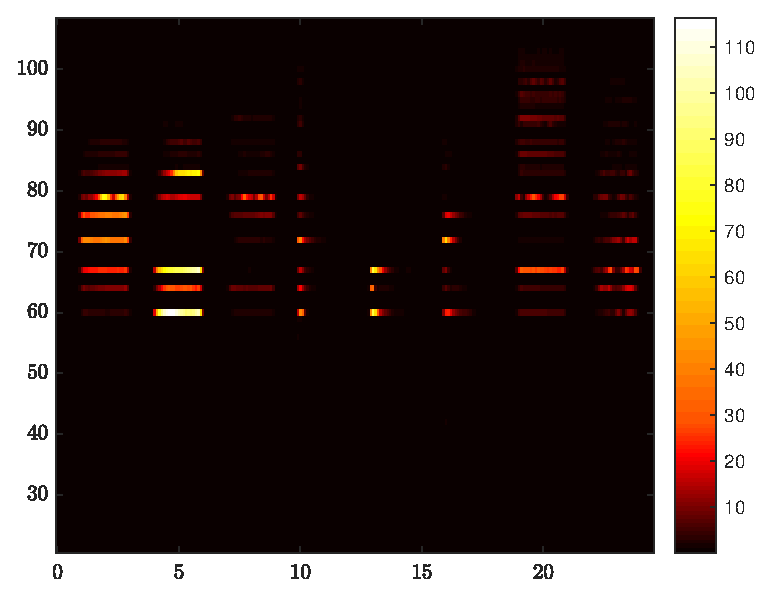
\includegraphics[width=0.4\linewidth]{img/PitchExample}
		\label{fig:PitchExample}
	}
	\hfill
	\subfigure[Example of CENS features]{
		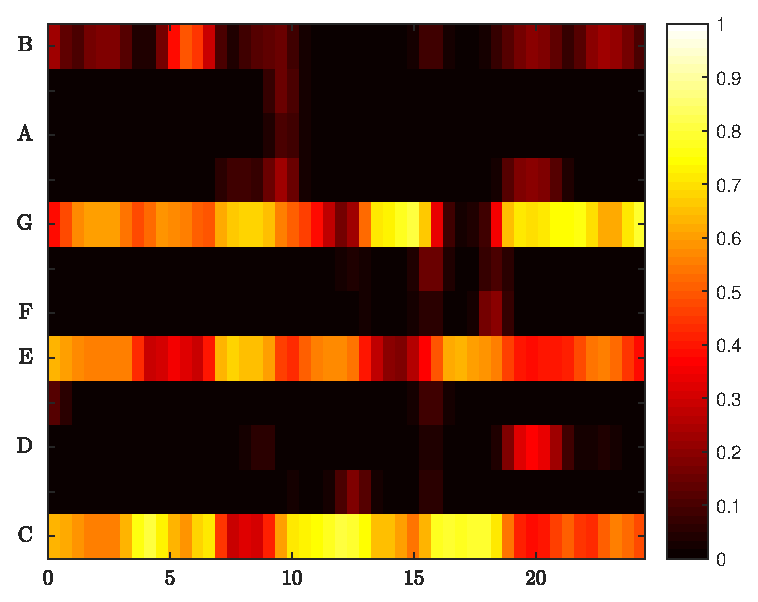
\includegraphics[width=0.4\linewidth]{img/CENSexample}
		\label{fig:CENSexample}
	}
	\hfill
	\vspace{-4mm}
	\caption{Example of feature extraction from a track containing the same chord played by 8 different instrument. You can see in \subref{fig:PitchExample} the different harmonic content while in \subref{fig:CENSexample} the instruments are basically indistinguishable}
	\label{fig:exampleChromaToolbox}
	\vspace{-5mm}
\end{figure*}
%
Feature extraction is performed using \textit{Chroma Toolbox} \cite{ChromaToolbox}, a MATLAB implementation of many different audio/musical features under GPL license.

At first, the audio signal is decomposed into 88 frequency bands centered in the frequencies corresponding to the pitches of notes A0 up to C8. A multirate filter bank using elliptic filters is used and finally \textit{Short-Time Mean-Square Power} (STMSP) is used to extract the useful information. In order to ignore the different harmonic profiles given by different instruments, the energies referred to the same notes are pooled together resulting in 12-dimensional vectors.

The different features are then obtained operating in different ways on the extracted pitches. In this project we used three of them:
\begin{itemize}[noitemsep,nolistsep]
	\item CLP (\textit{Chroma Features with Logarithmic Compression}): bands from different octaves are summed together, a logarithmic function is applied (to emulate our logarithmic perception of sound intensity) and then the vector is normalized in $L_2$-norm.
	\item CENS (\textit{Chroma Energy Normalized Statistics}): in order to account for dynamics, timbre, articulation, execution of note groups, and temporal micro-deviations, smart logarithmic quantization, temporal smoothing, downsampling and normalizations are performed.
	\item CRP (\textit{Chroma DCT-Reduced log Pitch}): they include logarithmic compression, smoothing and timbre invariance by using a DCT-based technique.
\end{itemize}
\subsection{Template-based chord recognition}
\label{subsec:templates}

Template matching consists of two steps: first, the templates are computed and second, the distance between the extracted features and the templates is calculated. In this project two types of templates are used: the \textit{binary templates} and the \textit{harmonic templates}. Binary templates are a simple binary representation of the chords (0 if the note is not present, $1/\sqrt{3}$ if the note is present). In order to create more accurate templates, the harmonics of each chord's note are also taken in count for the harmonic templates.

Adopting techniques taken from \cite{gomez2006tonal},\cite{oudre2009chord}, the first 6 harmonics of each note where used, exponentially attenuating each successive harmonic of each note (i.e. multiplying the harmonics by $[1, s, s^2, s^3, s^4, s^5]$, with the suggested factor $s=0.6$) and finally adding everything up and normalizing the result.
\subsection{Gaussian Mixture Models (GMMs)}
\label{subsec:gmm}

\textit{Gaussian Mixture Models} are a statistic technique used to individue subpopolations within an overall population. At the end of the process, each subpopulation is assigned to a \gls{mgd}.  As it is widely knows, \gls{mgd} is defined only by a mean vector and a covariance matrix. We notice that given a \gls{mgd} it is very simple determine the probability of that an object belongs to the distribution. We just need to implement the \textit{Mahalanobis distance} which measures how many standard deviations the selected object is distant from the distribution mean. \\
%
MATLAB defines a class called \textit{gmdistribution} which allows to construct an object that contain one or more \gls{mgd}s. This object can be built either by adding every distributions by ourself (supervised method) or fitting the entire population with a chosen number of distributions (unsupervised method). MATLAB offers also the method \textit{mahal} to compute the Mahalanobis distance between an object $X$ and a GMM. \\
%
GMMs represent a very simple and effective technique, which can be easily implemented with the pre-established MATLAB methods. In our work we focus on the supervised approach of GMM, creating the singles subpopulations one at time during the training phase.

\subsection{Multiclass Support Vector Machines (MC-SVM)}
\label{subsec:svm}

\textit{Support Vector Machines} (SVM) are a well known and widely used \textit{Machine Learning} algorithm for binary classification. Before \textit{Neural Networks} (NN) became so popular, they generally outperformed most of the other standard classification algorithms. Some good advantages over them is the possibility of choosing non-linear kernels (the most famous ones are the \textit{Gaussian/RBF} and the \textit{Polynomial}). Also, they are far easier to use and optimize than NN (less hyperparameters) and they tend to overfit less.\\
%
Their main problem, though, is that they were conceived for binary classification. Their extension to multiclass classification is not trivial but there are some standards ways to do it. One of them is already implemented in MATLAB and it's called \textit{Error-Correcting Output Codes} (ECOC). It works by creating multiple classifiers and assigning to each of them some classes to be considered positive and some other to be negative and by assigning weights to these binary classifiers, the final decision is taken.\\
%
For our tests we used the \textit{One-vs-One} method, meaning that we create a classifier for every couple of classes ($O(K^2)$) assigning one class to the positive and one to the negative, while ignoring everything else. This is usually a good trade-off between complexity and precision, but other options could be explored in future works.
\subsection{Hidden Markov Models (HMMs)}
\label{subsec:hmm}

\textit{Hidden Markov Model} represents an extremely powerful technique that has been widely used in speech recognition application for twenty years. A HMM consistis in an extension of the classical Markov Model scenario, in which observations are considered probabilistic functions of states. The final result is a pair of stochastic processes connected to each other; one process is directly observable, the other process is not and therefore is called "hidden". A more detailed theory about HMM working can be found in \cite{LawrenceHMMtutorial}. \\
%
In the speech recognition field HMMs are used as statistical method in order to recover specific sequences of sound. The validity of HMMs in the the particular case of chord transcription has already been demostrated in numerous papers including \cite{AlexDanEMplusHMM} and \cite{belpickMusic}. Both these work utilize the HMM approach proposed in \cite{GoldMorganSpeechRecogn}, training HMM with the \textit{Expectation-Maximization Algorithm}. As this work is not limited to implementing HMM, we choose to take a different approach. In particular we combine HMM to the SVM technique previously presented. \\
%
As suggested in \cite{GoldMorganSpeechRecogn} the working of HMM can be supported by the \textit{Viterbi Algorithm}. This algorithm aims to find the most likely sequence of states given the sequence of observables in a HMM scenario. It works in a recursive mode, first finding the probability of each HMM state for each observable, then identyfing the most probable states sequence. Given a total number of states equal to $N$ and a sequence of observables $T$ long, the Viterbi algorithm shows a complexity equal to $O(T \times N^2)$. The implementation of Viterbi algorithm represents the most difficult challenge in the HMM approach. Codes already existing often raise problems and therefore need to be carefully adapted to our scenario.

\section{Experiment Setup}
\label{sec:setup}

Our experimentation was split in two parts: the first was about recognizing a single chord from a single chord track, the second one was about recognizing the chords of full songs.\\
%
For the first part, we used the dataset \texttt{jim2012Chords} \cite{jim2012Chords} created for their paper \cite{JimChordsPaper}. It's composed of a total of over $2.000$ recordings of 10 guitar chords (both major and minor triads). Four different Guitars are used, as well as Piano, Violin and Accordion. Some tracks were recorded in an anechoic chamber, some other in a noisy environment. For each one of the tracks we obtain a 12-dimensional feature vector using \textit{Chroma Toolbox} and taking the maximum value for each note. Looking at Fig.~\ref{fig:CENSexample}, the idea is that we are interested in high values of specific groups of notes in order to guess the chord and the maximum value is a simple way of doing this. It's biggest disadvantage is that impulsive noisy environment can easily mask the useful information introducing high values in the wrong notes. Finally, we run the different methods on these obtained 12D vectors.\\
%
For the second part we used as dataset \textit{The Beatles}' discography, which has been professionally transcribed by Christopher Harte. This dataset contains the chords transcription of all The Betales's songs. Harte's work has proven to be extremely high quality and is an excellent resource for speech processing research. Details on how the chords transcription was achieved can be found in \cite{HartePaper} and in \cite{HarteThesis}. In his work Harte performed a very detailed transcription, obtaining a wide set of chords. For reduce computational cost we mapped the labels transcripted by Harte into $24$ labels, which coincide with the $12$ notes of the chromatic scale in the major and minor version. For similar reason we selected only $150$ Beatles songs out the $180$ trasncribed by Harte, keeping anyway a big number of songs to work on. From now on, we indicate our labels dataset with $\Lambda$ and our songs dataset with $\mathcal{D}_{Beatles}$. \\
%
The second part of the experiment was divided in three steps which are \textit{pre-processing}, \textit{training} and \textit{testing}. As machine learning approach, we randomly divided our dataset in two subset that we call \textit{training dataset} $\mathcal{D}_{train}$ and \textit{testing dataset}  $\mathcal{D}_{test}$. We call $r_{train}$ the ratio between $|\mathcal{D}_{train}|$ and $|\mathcal{D}_{Beatles}|$ and $r_{test}$ the ratio between $|\mathcal{D}_{train}|$ and $|\mathcal{D}_{Beatles}|$. During the experiment we varied the value of $r_{test} \in \{0.1,0.2,0.3\}$, consequently obtaining $r_{train}$ as $1-r_{test}$. Every song of both the subsets was processed according to one of the technique offered by \textit{Chorma toolbox}. We noticed that we set toolbox parameters so that we didn't get an exaggerated number of frames per song. In \textit{results} section we will see that this choice could make outputs weaker, especially in CLP and CRP cases. After features extraction was completed, we obtained a sequence of \textit{frame-features} for each song in $\mathcal{D}_{Beatles}$; the length of the sequence depended both on the song duration and the chosen featuring process $(CENS,CLP,CRP)$. Harte's work gave us information about the chord periods in each songs; we wanted to make compatible this information with the data obtained by features extraction. With this purpose we divided the periods computed by Harte in sub-periods with equal time-length to the frames computed with Chroma toolbox. For each song we obtained a sequence of \textit{frame-labels} with equal length to the sequence of \textit{frame-features}; from now on we indicate the \textit{frame-labels} sequence for a generic song with $\mathcal{L}_{Harte}$. Finally we noticed that almost all the songs presented periods with no sounds; in the dataset these period were marked with the '$N$' label. Obviously '$N$' frames were out of our interested and therefore were discarded. \\
%
At the end of the \textit{pre-processing} phase we obtained two sets of songs $(\mathcal{D}_{train},\mathcal{D}_{test})$, in wich every songs is assigned to both a sequence of \textit{frame-features} and a sequence of \textit{frame-labels}. The data contained in $\mathcal{D}_{train}$ were then used to train the MC-SVM and subsequently build the HMM. MC-SVM training was achieved using one chord at time, as done in the first part of the experiment, and using as kernel the \textit{polynomial} one. HMM training was achieved testing the data contained in $\mathcal{D}_{train}$ with the MC-SVM previously built. The resulting errors of this process allowed us to establish values for the \textit{emission probabilities}. Analyzing directly all the $\mathcal{L}_{Harte}$ \textit{transition probabilities} and \textit{initial probabilities} values were computed. \\
%
Once all our methods were trained, the \textit{testing} began. We took the \textit{frame-features} of $\mathcal{D}_{test}$ and we processed them first only with MC-SVM methods, then also with HMM. Therefore for each song we obtained two different outputs, that we call $\mathcal{L}_{SVM}$ and $\mathcal{L}_{HMM}$. $\mathcal{L}_{SVM}$ corresponds to the \textit{frame-labels} sequence produced by the MC-SVM. In this process every frame was assigned to a chord, without taking in account the others frame componing the song.  $\mathcal{L}_{HMM}$ corresponds to the \textit{frame-labels} sequence produced by the HMM, which took MC-SVM's output and tried to improve it. The HMM's output was obtained implementing the Viterbi algorithm, which allowed to taking into account the whole sequence of chords that compone the song.

\section{Results}
\label{sec:results}

\begin{table}[t]
	\centering
	\begin{tabular}{|c|ccc|}
		\hline
		Classification & CLP & CENS & CRP \\
		\hline
		Template (binary) & 24.17\% & 20.08\% & 24.96\% \\
		Template (harmonic) & 23.04\% & 17.79\% & 20.38\% \\
		GMM & 14.58\% & 6.94\% & 11.81\% \\
		\hline
		SVM (linear) & 13.61\% & 6.39\% & 12.64\% \\
		SVM (poly) & 10.56\% & 4.17\% & 7.92\% \\
		SVM (RBF) & 10.00\% & 4.31\% & 7.78\% \\
		\hline
	\end{tabular}
	\caption{Error results of the first part of the tests (single chord recognition).}
	\label{tab:singleChordResults}
\end{table}

For the first part of the experiment we simply run all the different classification methods explained in Section~\ref{sec:setup} randomly splitting the dataset into $70\%$ training and $30\%$ testing. The results can be clearly seen in Tab.~\ref{tab:singleChordResults}. Note that the first approach (templates) yields very poor results even in such an idealized scenario, although the more advanced \textit{Harmonic Templates} improve a little bit performance over the simple \textit{Binary} ones. The jump to the more advanced GMMs is pretty clear as much as the one to SVMs. Overall, CENS features have by far the best error rates.

For the second part of the experiment we got two different kind of outputs for each song, which are $\mathcal{L}_{SVM}$ and $\mathcal{L}_{HMM}$. In order to verify the quality of ours results we compared them with  $\mathcal{L}_{Harte}$. Given $\mathcal{L}_{SVM}$ ($\mathcal{L}_{HMM}$) and $\mathcal{L}_{Harte}$ for a certain value of $r_{test}$ and for a certain extracted feature we computed the error probability counting all the matching between $\mathcal{L}_{SVM}$ ($\mathcal{L}_{HMM}$) and $\mathcal{L}_{Harte}$.

 In Tab.~\ref{tab:resultbeforeHMM} we can look at the error probabilities obtained after the first step of testing, before processing HMM. In Tab.~\ref{tab:resultafterHMM} we can look at the results obtained after the second step of testing, after processing HMM. In both cases we show different outputs depending on the testing rate $r_{test}$ and on the chosen extracted feature.

\begin{table}[h!]
	\caption{Results of the second part before processing HMM}
	\centering
	\begin{tabular}{|c |c c c|}
	\hline
	$r_{test}$ & CENS & CLP & CRP\\ \hline
	0.1 & 49.46\% & 47.39\% & 62.06\%\\
	0.2 & 46.57\% & 60.00\% & 63.76\%\\
	0.3 & 47.65\% & 56.91\% & 58.03\%\\
	\hline
	\end{tabular}
	\label{tab:resultbeforeHMM}
\end{table}

\begin{table}[h!]
	\caption{Results of the second parts after processing HMM}
	\centering
	\begin{tabular}{|c |c c c|}
	\hline
	$r_{test}$ & CENS & CLP & CRP\\ \hline
	0.1 & 44.39\% & 45.02\% & 56.41\%\\
	0.2 & 42.96\% & 59.19\% & 59.67\%\\
	0.3 & 41.79\% & 54.84\% & 52.04\%\\
	\hline
	\end{tabular}
	\label{tab:resultafterHMM}
\end{table}

 Observing the results we make the following observations. First, we got best results with CENS features than with CLP and CRP features. This is reasonable since also in the first part of the experiment we got better results with CENS than others type of features. Second, HMM proved to be able to enhance better results than MC-SVM alone in all the cases. This is not obvious since we worked with features of multi-instrumental sounds including also vocal parts. Indeed the chords prediction of some songs often isn't improved but is aggravated. We show this by comparing the two different results obtained with the same $\mathcal{D}_{train}$ as done in Fig.~\ref{fig:compareerror}.

\begin{figure} [h!]
	\centering
	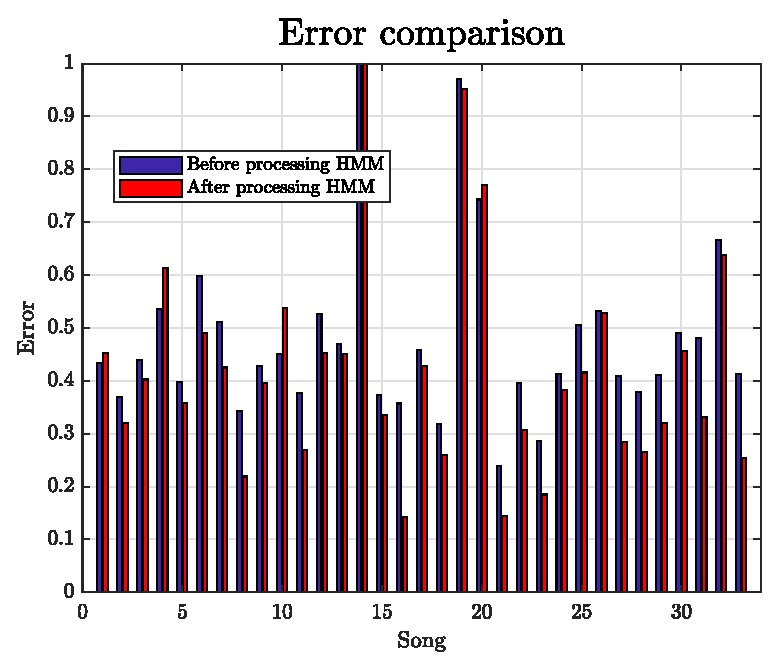
\includegraphics[width=0.45\textwidth]{img/Result_HMM/CENS/plot03071}
	\caption{Error comparison using CENS features and $r_{test}=0.3$}
	\label{fig:compareerror}
\end{figure}

We concluded that HMM don't always improve our result for every single song. It is able to do so only in average. However what HMM is able to do for each song is reduce the chords variation. We define chord variation as the number of times that a chord sequence varies within the same song, therefore the number of times that $\mathcal{L}(i) \neq \mathcal{L}(i-1)$. This value decreases, since HMM tends to correct the most improbables outputs generated by MC-SVM. We find confirmation to this assumption looking at
Fig.~\ref{fig:smoothmulti} and Fig.~\ref{fig:smoothsingle}. In particular in Fig.~\ref{fig:smoothsingle} we can see how HMM removes the chord-labels that are not repeated costantly over time and therefore result less likely.

\begin{figure} [h!]
	\centering
	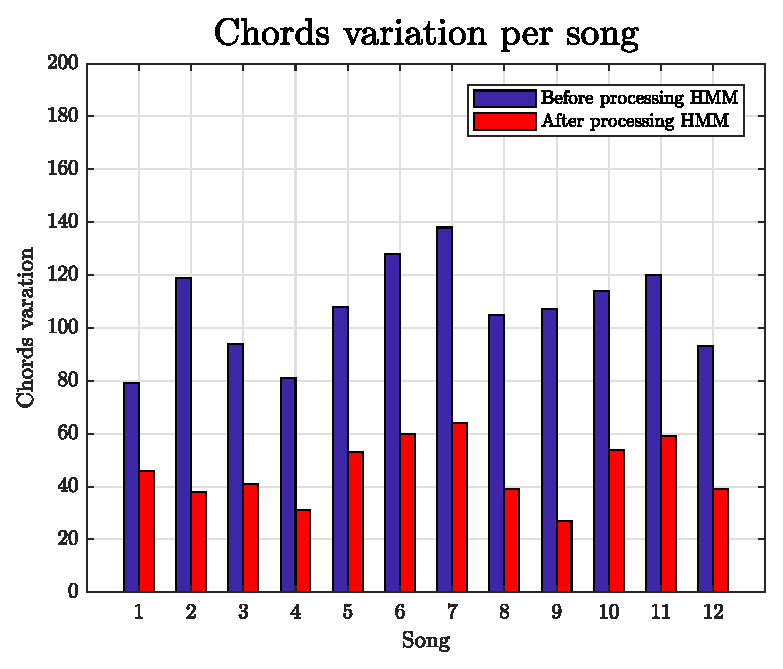
\includegraphics[width=0.45\textwidth]{img/Result_HMM/SMOOTHING/SmoothPerSongCENS0109}
	\caption{Chords variation per song using CENS features and $r_{test}=0.1$}
	\label{fig:smoothmulti}
\end{figure}

\begin{figure} [h!]
	\centering
	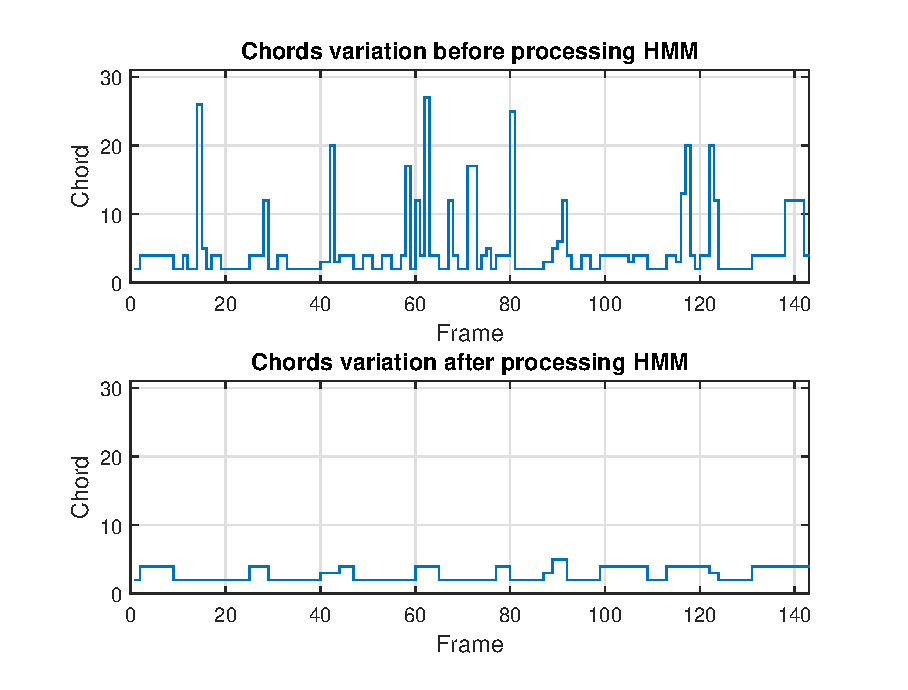
\includegraphics[width=0.45\textwidth]{img/Result_HMM/SMOOTHING/SmoothSingleSongCENS0109}
	\caption{Chord variation in a single song using CENS features and $r_{test}=0.1$}
	\label{fig:smoothsingle}
\end{figure}

\section{Conclusions}
\label{sec:conclusions}

After seeing the results in Sec.~\ref{sec:results}, it should be clear that the more advanced techniques described in Sec.~\ref{sec:techniques} improve the results very significantly over the oldest and simplest ones.

In particular, CENS features are able to perform really well with all classifiers but the most advanced ones (SVM with non-linear kernels) clearly outperform all the others.

Using this information, we tried to predict chords in full songs having, of course, poorer results, due to the increased complexity of the problem. The HMM-based approach, again, was able to improve performance over the trivial \textit{per-frame} one.

Future works might try to use different type of features and classifiers for the general chord recognition problem, as well as exploring the hyperparameters given by the ECOC for the multiclass SVM classifier. When dealing with entire songs, instead, it might be useful to either extract or subtract specific instruments (e.g. drums) and voice, since we believe they are the main cause of the high error rates obtained.

% References should be produced using the bibtex program from suitable
% BiBTeX files (here: strings, refs, manuals). The IEEEbib.bst bibliography
% style file from IEEE produces unsorted bibliography list.
% -------------------------------------------------------------------------
\bibliographystyle{IEEEbib}
\bibliography{bibliography}

\end{document}
